\chapter{Crittografia su curve ellittiche}
Attorno al 1985 Miller (IBM, non lo stesso Miller di Miller-Rabin) e Koblitz (University of Washington) propongono di prendere RSA e DH e cambiare le operazioni in algebra modulare con operazioni su curve ellittiche.
\paragraph{Wait} Prima di introdurre il cifrario è necessario entrare nel concetto di \emph{curva ellittica}.

\section{Vantaggi della crittografia a curve ellittiche}
Si sta via via abbandonando la crittografia basata sull'algebra modulare per abbracciare operazioni definite sui punti di una \emph{curva ellittica}: 
\begin{itemize}
	\item le chiavi risultano più piccole a parità di sicurezza;
	\item fattorizzazione e logaritmo discreto si risolvono in tempi sub-esponenziali.
\end{itemize}
Gli algoritmi per rompere la cifratura su curve ellittiche rimangono ad ora ancora esponenziali puri (anche qua vale l'approccio delle funzioni \emph{one-way trap-door}).
\begin{table}[ht]
    \centering
    \begin{tabular}{c|c|c}
        AES & RSA, DH, El Gamal & ECC \\
        \hline
        128 bit & 3072 bit ($n$ per RSA, $p$ per DH) & 256 bit \\
        256 bit & $\approx 15'000$ bit & 512 bit
    \end{tabular}
\end{table}

\noindent Il fatto è che ECC ECC (\emph{Elliptic Curve Cryptography}) offre la stessa sicurezza di RSA, ma con un numero di bit decisamente inferiore! Logicamente ci piace di più un cifrario che richiede una minore occupazione di memoria.

\section{Curve ellittiche}
\paragraph{Definizione di campo} \emph{Il campo $K$ è un insieme non vuoto dotato di operazioni binarie interne, chiamate addizione e sottrazione, che soddisfano la proprietà associativa, commutativa, di esistenza dell'elemento neutro e di esistenza dell'inverso di ciascun elemento (ad eccezione dello zero per la moltiplicazione)}. 
\paragraph{Forma generale} Preso un campo $K$ una curva ellittica è l'insieme dei punti $(x,y) \in K^2$ tale che:
$$ y^2 + axy + by = x^3 + cx^2 + dx + e $$
con $a,b,c,d,e \in K$.

\paragraph{Definizione di caratteristica del campo} La caratteristica di un campo è il numero di volte per il quale devo sommare l'elemento neutro moltiplicativo $1$ per ottenere l'elemento neutro additivo $0$.
\begin{itemize}
	\item Negli interi modulo $p$ la caratteristica è $p$.
	\item Nei reali la caratteristica è 0 (non esistono numeri in grado di fare quanto detto).
\end{itemize}

\paragraph{Forma normale di Weierstrass} Se la caratteristica di $K \neq 2, 3$ allora esiste una forma semplificata:
$$ y^2 = x^3 + ax + b $$
con $a,b \in K$. Scriviamo quindi:
$$ E_K = \{ (x,y) \in K^2 \mid y^2 = x^3 + ax +b \} \cup \{0\} $$
Si osservi che introduciamo l'elemento neutro $0$ dell'operazione (quella che stiamo costruendo), uniamo all'insieme di punti un elemento 0 che in base al campo può già esistere o meno. Sarà per noi un punto all'infinito.
\paragraph{Gruppo Abeliano} All'interno di $E(a,b)$ possiamo definire una operazione interna, dando all'insieme la struttura algebrica di un \emph{gruppo Abeliano}: ci limitiamo a questo, non andiamo a definire un campo vero e proprio (le proprietà presenti sono inferiori rispetto a quelle della definizione di campo). 

%\paragraph{Attenzione} Non tutte le curve ellittiche hanno la struttura di gruppo Abeliano!


\section{Curve ellittiche su $K=\mathbb{R}$}
\paragraph{Radice} \emph{Sia $K$ un campo. Un elemento $a \in K$ si dice radice, o zero, di un polinomio $f(x)$ a coefficienti in $K$ se: $f(a) = 0$} (da \url{http://progettomatematica.dm.unibo.it/}).

\paragraph{Radice multipla} \emph{Una radice di un polinomio è detta multipla se ha molteplicità maggiore di $1$} (da \url{http://progettomatematica.dm.unibo.it/}).

\paragraph{Definizione} La definizione è quella già introdotta:
$$ E_{\mathbb{R}}(a,b) = \{(x,y) \in \mathbb{R}^2 \mid y^2 = x^3 + ax +b \} \cup \{0\} $$
Per avere un gruppo Abeliano in $\mathbb{R}$ è necessario che $x^3 + ax + b$ non abbia radici multiple, quindi si assume che:
$$ 4a^3 + 27b^2 \neq 0 $$
Questo ci garantisce l'assenza di radici multiple. L'assenza di radici multiple garantisce l'assenza di punti singolari, quindi esiste sempre la tangente esiste in ogni punto della curva ellittica.
\paragraph{Esempi di curve ellittiche}
\begin{center}
    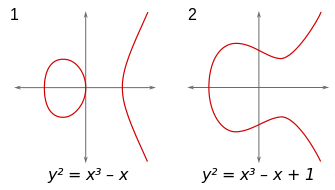
\includegraphics[width=225px]{images/ECC_1.png}
\end{center}
Sulla sinistra una curva a due componenti, sulla destra una curva ad una componente.
Si osservi le radici della cubica $x^3 + ax +b$, si hanno tre radici che possono essere:
\begin{itemize}
    \item 3 reali $\implies$ Curva a due componenti
    \item 1 reale e 2 complesse coniugate $\implies$ Curva ad una componente
\end{itemize}
 {{Si noti che le curve ellittiche sono sempre simmetriche rispetto all'asse delle $x$}}. Se non imponessimo radici distinte avremmo curve con cuspidi o con nodi, in queste particolari curve la tangente non è detto che esista unica (e questa cosa ci serve).

\subsection{Punto opposto $\mathbf{-P}$} La simmetria viene dal termine $y^2$, infatti:
$$ P = (x,y) \in E(a,b) \implies y^2 = x^3 + ax + b $$
definiamo dunque:
$$ -P = (x,-y) \implies (-y)^2 = y^2 = x^3 + ax + b $$
Dato $P=(x,y) \in E(a,b) $ si dice \emph{opposto} e si indica con $-P$ il punto $-P=(x,-y)$. Per il punto all'infinito si pone $0=-0$.

\subsection{Somma sulla curva ellittica}
Vogliamo definire un nuovo sistema a chiave pubblica, per fare ciò serve una funzione \emph{one-way trap-door}. Per avere una funzione per prima cosa dobbiamo definire un'operazione sull'insieme dei punti. Definiamo la \textit{somma} (attenzione, non ha nulla a che fare con la somma delle coordinate!
\paragraph{Cosa facciamo?} Facciamo l'intersezione tra la curva ellittica e una retta
\[
\begin{cases}
	y = mx + q \\
	y^2 = x^3 + ax + b
\end{cases}
\]
manipolando le equazioni mi trovo con una cubica della $x$. Le situazioni possibili sono:
\begin{itemize}
	\item un solo punto reale e due complessi coniugati;
	\item tre reali.
\end{itemize} 
Posso avere al massimo tre punti di intersezione.  Posso quindi prendere due punti sulla curva P e Q dato che ho due intersezioni esplicite ce ne sarà una terza per forza, chiamiamolo $R$. Il risultato di questa somma sarà $-R$ (per definizione).
\begin{center}
    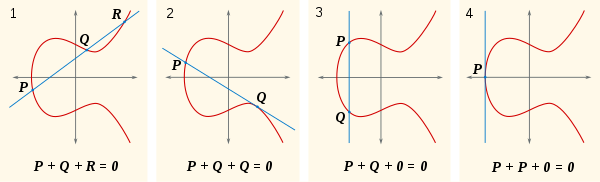
\includegraphics[width=390px]{images/ECC_2.png}
\end{center}

\subsubsection{Definizione di somma} Presi $P, Q, R \in E(a,b)$ se $P, Q, R$ sono disposti su una retta si pone:
$$ P + Q + R = 0 \implies P + Q = -R $$
\begin{center}
	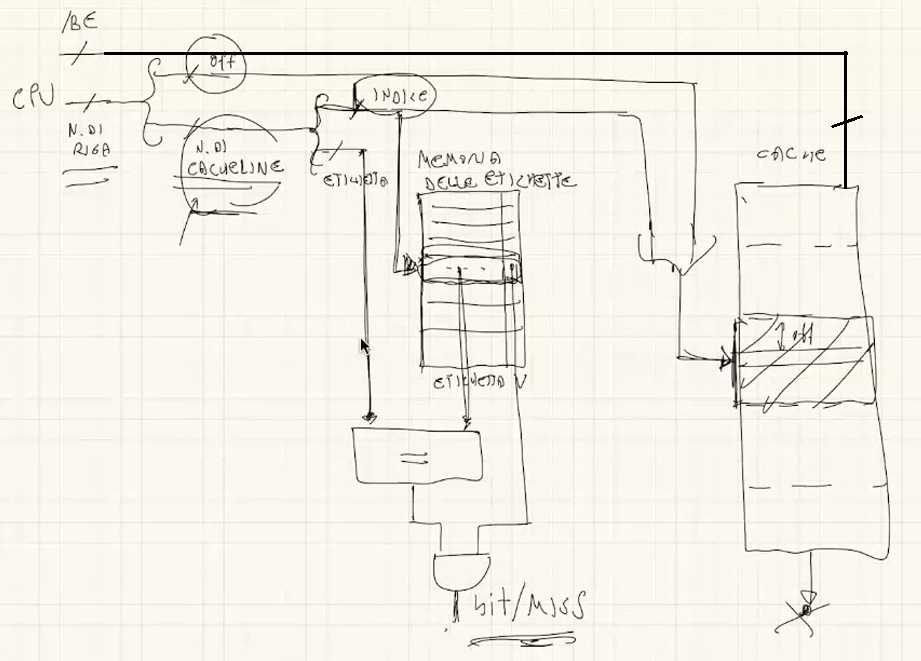
\includegraphics[scale=.8]{images/28.png}
\end{center}
Distinguiamo i vari casi:
\begin{itemize}
	\item $\mathbf{Q \neq \pm P}$. I punti $P, Q \in E(a,b)$. Trovo il terzo punto $R \in E(a,b)$ e utilizzo la formula della definizione. Nessun problema poichè $-R \in E(a,b)$
	\item Se $\mathbf{Q=-P}$ sommiamo il punto con il suo opposto
	$$P+(-P)=-0=0$$
	Si ricordi che nella nostra operazione l'elemento neutro è il punto all'infinito (si veda la terza figura prima della def.). 
	\item Se $\mathbf{Q = P}$ si considera la tangente alla curva nel punto $P$ (sempre definita per costruzione in quanto $4a^3+2tb^2 \neq 0$) e se ne vede l'intersezione con la curva. Si prende l'opposto del punto di intersezione tra tangente in $P$ e curva (può essere $O$).
	\begin{center}
		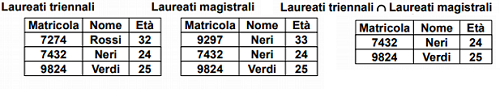
\includegraphics[scale=.85]{images/29.png}
	\end{center}
	Si noti che anche in questo caso se si fa passare una retta sull'estremo sinistro si ha una retta verticale e quindi la somma può dare il punto all'infinito (si veda la quarta figura prima della def.).
\end{itemize}

\subsubsection{Proprietà della somma}
\begin{itemize}
	\item \textbf{Chiusura}. $\forall P, Q \in E(a,b): P+Q \in E(a,b) $
	
	Dalla somma di due elementi otteniamo sempre un terzo elemento appartenente alla curva. 
	
	\item \textbf{Elemento neutro}. $ \forall P \in E(a,b): P + 0 = 0 + P = P $
	
	Per ogni punto appartenente alla curva ellittica esiste l'elemento neutro, ossia un punto che sommato al primo non lo altera.
	
	\textbf{NB}: Prendendo un punto $P$ e tracciando la retta all'infinito passante per $P$ l'altra intersezione è $-P$ quindi il risultato è $-(-P) = P$.
	
	\item \textbf{Inverso (opposto)}. $$ \forall P \in E(a,b)\,\, \exists! \, Q \in E(a,b) : P + Q = 0 = Q + P$$
	$$ Q = -P \implies P = (x,y), Q = (x, -y) $$ 
	
	Per ogni punto $P$ appartenente alla curva ellittica esiste uno e un solo punto $Q$ tale che $P+Q=0$
	
	\item \textbf{Commutativa}. $\forall P, Q \in E(a,b) P + Q = Q + P $
	
	\item \textbf{Associativa}. $ \forall P, Q, R \in E(a,b):\, (P + Q) + R = P + (Q + R) $
\end{itemize}

\subsubsection{Formulazione algebrica}
Dati \begin{align*}
	P = (x_P, y_P)&&Q = (x_Q, y_Q)&&S = (x_S, y_S) = P+Q
\end{align*}
abbiamo:
\begin{itemize}
    \item $\mathbf{Q \neq \pm P}$:
    \[
        \begin{cases}
        	\lambda = \frac{y_Q - y_P}{x_Q - x_P}\\
            x_S = \lambda^{2} - x_P - x_Q \\
            y_S = \lambda(x_P - x_S) -y_P 
        \end{cases}
    \]
    \item $\mathbf{P = Q}$:
    \[
        \begin{cases}
        	\lambda = \frac{3x_P^{2} + a}{2y_P}\\
            x_S = \lambda^{2} - x_P - x_Q \\
            y_S = \lambda(x_P - x_S)-y_P 
        \end{cases}
    \]
    
    NB: se $y_P = 0$ allora $P+P=0$
    \item $\mathbf{Q = -P}$: otteniamo il p.to all'infinito $$P+Q = 0$$
\end{itemize}

\section{Curve ellittiche su campi finiti}
In crittografia non possiamo usare le curve su campi reali: la crittografia ha bisogno di un'aritmetica veloce e assolutamente precisa (senza, ad esempio, errori di arrotondamento). Quello che facciamo è prendere curve definite su campi finiti (quindi un numero finito di elementi): vedremo le cosiddette \emph{curve prime}. 
\begin{itemize}
	\item Il campo è l'insieme $\mathbb{Z}_p=\{0,1,\dots,p-1\}$
	\item $p$ è numero primo
	\item La caratteristica di $\mathbb{Z}_p$ è $p$. 
	\item Imponiamo $p>3$ per poter utilizzare la forma normale di Weierstrass.
\end{itemize}
Non abbiamo più una figura continua, ma una nuvola di punti (cit.)! Noi consideriamo solo le curve prime per le quali $4a^3 + 27b^2 \text{ mod } p \neq 0$ (CNS per gruppo Abeliano).
\paragraph{Campo} Ridefiniamo quindi la curva:
$$ E_p(a,b) = \{ (x,y) \in Z_p^2 \mid y^2 \text{ mod } p = (x^3 + ax + b) \text{ mod } p \} \cup \{0\} $$
\begin{itemize}
	\item Si noti che essendo in modulo si lavora sempre nel primo quadrante: $x \geq 0, y \geq 0$.
	\item La curva sarà ancora simmetrica ma non rispetto a  $y = 0$, bensì rispetto $y = \lfloor \frac{p}{2} 	\rfloor$
	\item Inoltre tutti i valori saranno in $[0, p-1]$ per il modulo (elementi appartenenti a $\mathbb{Z}_p$).
	\pagebreak 
	\item Essendo simmetrica se $P=(x,y) \in E_p(a,b)$ allora
	$$-P = (x, p-y) \in E_p(a, b)$$
	Se $y^2 \equiv x^3 + ax + b$ allora $(p-y)^2 \equiv p^2 -2py + y^2 \equiv y^2$ poichè $p$ è lo zero nel campo.
\end{itemize}
Le formule della somma sono dunque le stesse ma si lavora in modulo (le divisioni diventano moltiplicazioni per l'inverso se non ci sono semplificazioni immediate, l'inverso c'è sempre perché lavoriamo modulo un numero primo). 
\begin{center}
	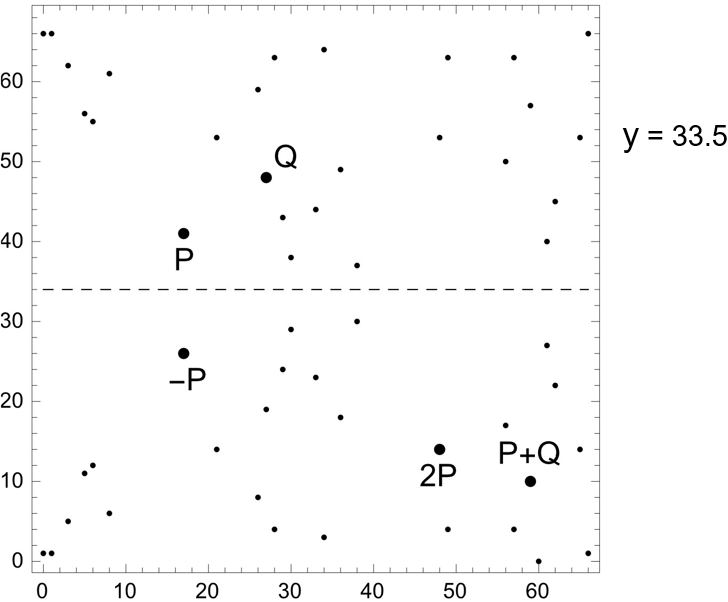
\includegraphics[scale=.5]{images/32.PNG}
\end{center}
\paragraph{Esempio} Prendiamo $P=(17,41) \in E_{67}(-1,1)$. L'elemento è rappresentato in figura. Calcoliamo l'opposto:
$$-P=(17,-41 \text{ mod }67)=(17, -41+67)=(17,26) \in E_{67}(-1,1)$$
La condizione per definire un gruppo Abeliano è valida: $(4a^3+27b^2) \text{ mod } p \neq 0$
\subsection{Formulazione algebrica}
Siamo nell'insieme $\mathbb{Z}_p$. Dati \begin{align*}
	P = (x_P, y_P)&&Q = (x_Q, y_Q)&&S = (x_S, y_S) = P+Q
\end{align*}
abbiamo:
\begin{itemize}
	\item $\mathbf{Q \neq \pm P}$:
	\[
	\begin{cases}
		\lambda = \frac{y_Q - y_P}{x_Q - x_P}\text{ mod } p\\
		x_S = (\lambda^{2} - x_P - x_Q)\text{ mod } p \\
		y_S = (\lambda(x_P - x_S) -y_P)\text{ mod } p 
	\end{cases}
	\]
	\item $\mathbf{P = Q}$:
	\[
	\begin{cases}
		\lambda = \frac{3x_P^{2} + a}{2y_P}\text{ mod } p\\
		x_S = (\lambda^{2} - x_P - x_Q)\text{ mod } p \\
		y_S = (\lambda(x_P - x_S)-y_P)\text{ mod } p 
	\end{cases}
	\]
\end{itemize}

\subsection{Ordine di una curva ellittica (cardinalità)}

\paragraph{Premessa} Cosa intendiamo con \emph{residuo quadratico}? Intendiamo un numero intero $q$ se esiste un intero $x$ tale che
$$x^2 \equiv q \text{ mod }p \longrightarrow x^2 \text{ mod } p = q$$

\paragraph{Definizione} L'ordine di una curva è il numero di punti che la curva possiede.
$$y^2=x^2+ax+b$$
Non esiste una formula precisa per trovare l'ordine: dipende dalla cubica. Prendo un valore $x\in \mathbb{Z}_p$
\begin{itemize}
	\item Si hanno al massimo $p$ valori per l'ascissa $x$, quindi mi aspetto circa $2p$ valori per l'ordinata $y$ (si ricordi che nella formula è posto il quadrato). Sommo $1$ per considerare il punto all'infinito:
	$$2p+1$$
	\item Non tutti i valori nel campo hanno una radice, quindi \textbf{\underline{sono molti meno}} di $2p + 1$.
	%\item In genere in $Z_p$ i residui quadratici che definiscono un punto sulla curva sono $\frac{p-1}{2}$.
	
	\item Il \textbf{teorema di {Hasse}} ci dice che se $N$ è l'ordine della curva prima $E_p(a,b)$ allora:
	$$ \mid N - (p+1) \mid \leq 2\sqrt{p}  $$
\end{itemize}
\paragraph{Esempio} Consideriamo la seguente curva
$$y^2\equiv (x^3+4x+4) \text{ mod }5$$
Calcoliamo i quadrati dei punti del campo, in modo da capire quali sono residui quadratici e quali no.
\begin{center}
	\begin{tabular}{c|c c c c c}
		\hline
		$y$ & 0&1&2&3&4  \\
		$y^2 \text{ mod }5$ & 0&1&4&4&1  \\
	\end{tabular}
\end{center}
Osserviamo che i numeri $0,1,4$ sono residui quadratici. Per la costruzione della curva consideriamo i possibili valori $x$.
\begin{align*}
	& \Longrightarrow y^2\equiv (x^3+4x+4) \text{ mod }5\\
	x=0 &\Longrightarrow y^2=4 \Longrightarrow (0,2), (0,3) \in E_5(4,4)\\
	x=1 &\Longrightarrow y^2=4 \Longrightarrow (1,2),(1,3) \in E_5(4,4)\\
	x=2 &\Longrightarrow y^2=0 \Longrightarrow (2,0) \in E_5(4,4)\\
	x=3 &\Longrightarrow y^2=3 \Longrightarrow \text{Non esistono punti di ascissa $3$}\\
	x=4 &\Longrightarrow y^2=4 \Longrightarrow (4,2),(4,3) \in E_5(4,4)
\end{align*}
Abbiamo $7$ punti, più il punto all'infinito: l'ordine è $8$.
\subsection{Costruzione di una funzione \emph{one-way trap-door}}
C'è una specie di parallelismo tra le operazioni in algebra modulare e le operazioni sulla curva ellittica:
\begin{itemize}
    \item la \textbf{moltiplicazione} (algebra modulare) diventa la \textbf{somma tra due punti} (curve ellittiche)
    \item l'\textbf{elevamento a potenza} $k$ (algebra modulare) diventa la \textbf{moltiplicazione di un punto per lo scalare} $k$ (curve ellittiche)
    \begin{align*}y^k=y \cdot y \cdot \dots \cdot y \Longrightarrow kP=P+P+\dots+P\end{align*}
\end{itemize}
La funzione deve essere one-way, quindi la moltiplicazione deve avere costo polinomiale. Non possiamo fare la somma $k$ volte: non è praticabile, abbiamo una complessità esponenziale rispetto alla dimensione di $k$ (algoritmo pseudopolinomiale, crescita lineare nel valore, crescita esponenziale nella dimensione). Per rendere il numero di operazioni proporzionale al logaritmo del valore ricorriamo a un'addattamento dell'algoritmo delle esponenziazioni veloce: \textbf{algoritmo dei raddoppi ripetuti}.

\subsubsection{Moltiplicazione scalare: algoritmo dei raddoppi ripetuti}
\paragraph{Operazione ed esempio} Calcolare $Q = kP$ è one-way. Dati i valori $k$ e $P$ è facile calcolare $Q$ (si fa in $O(\log k)$). Consideriamo un esempio:
\begin{align*}
	&Q=13P=(1+4+8)P\\
	&P \longrightarrow 2P \longrightarrow 2(2P)=4P \longrightarrow 2(4P)=8P
\end{align*}
Con 3 raddoppi calcoliamo $8P$. Concludiamo
$$Q=P+4P+8P=13P$$

\paragraph{Formalizzazione} 
\begin{enumerate}
	\item Dato $Q = kP$, riscrivo $k$ in notazione binaria: 
	\begin{align*}
		k = \sum_{i=0}^{t}k_i \cdot 2^i && k=(k_tk_{t-1}\dots k_2k_1k_0)
	\end{align*}
	Mi servono quindi il seguente numero di bit
	$$t+1 = \lfloor \log_2 k \rfloor + 1$$
	\item Si calcolano i vari raddoppi $$2P, 4P, \dots, 2^tP$$
	abbiamo $t$ raddoppi ciascuno come raddoppio del punto precedente.
	\item Si calcola $$Q = \sum_{i : k_i = 1} (2^iP)$$ in esattamente $t$ somme: $O(t) = O(\log_2 k)$ quindi lineare nella dimensione dell'input.
\end{enumerate}


\paragraph{Operazione inversa} Dati $P$ e $Q$, sulla curva $E_p(a,b)$, trovare il più piccolo $k$ tale che$$Q = kP$$
Non si conoscono algoritmi polinomiali (neanche  sub-exp) per risolvere il problema. Si parla di \emph{logaritmo discreto sulle curve ellittiche}.

\section{Protocollo Diffie-Hellman su curve ellittiche}
\paragraph{Premessa} Definiamo l'\emph{ordine di un punto} il più piccolo numero $n$ tale che
$$nB=0$$
\paragraph{Algoritmo}
\begin{itemize}
	\item Alice e Bob concordano una curva ellittica prima (che soddisfi la condizione di gruppo Abeliano) ed un punto $B$ della curva che abbia ordine molto grande. I punti e le curve sono già consigliate dal NIST, non si devono quindi creare da zero (come già visto nella versione dell'algebra modulare). Sono note e pubbliche.
	
	Il punto $B$ ottenuto è il generatore (ricordarsi cosa facevamo nella versione in algebra modulare: definizione di un intero primo e grande $p$ e di un generatore $g$).
	
	\item L'algoritmo prosegue così:
	\begin{enumerate}
		\item Alice genera un valore $n_A < n$ casuale, calcola $$P_A = n_AB$$ e lo invia in chiaro a Bob
		\item Bob riceve $P_A$. Genera un valore $n_B < n$ casuale, calcola $$P_B = n_BB$$ e lo invia in chiaro ad Alice
		\item Alice riceve $P_B$ e calcola $S = n_AP_B = n_An_BB$
		\item Bob riceve $P_A$ e calcola $S = n_BP_A = n_Bn_AB$
	\end{enumerate}
	ambo le parti hanno generato lo stesso $S$ e possono quindi generare la stessa chiave di sessione in vari modi (ad esempio $K = x_S \mod 256$).
\end{itemize}




\paragraph{Crittoanalista}
\begin{itemize}
	\item  Un crittoanalista non può fare nulla perché conosce $E_p(a,b), B, n, P_A, P_B$ ma non può trovare $n_A$ o $n_B$ se non risolvendo il problema del logaritmo discreto su curva ellittica.
	
	\item E' sempre possibile un attacco \emph{man-in-the-middle}: segue che la chiave va sempre estratta da un certificato!
	
	\item Il sistema col logaritmo discreto su curva ellittica è facile sulla macchina quantistica.
\end{itemize}


\section{Scambio di messaggi (equivalente di El-Gamal)}
\subsection{Algoritmo di Koblitz per la trasformazione del messaggio}
Per prima cosa bisogna preparare il messaggio in chiaro: deve essere trasformato in punto della curva ellittica. 
$$ m \xrightarrow{} P_m \in E_p(a,b) $$
\paragraph{Soluzione (sbagliata)}Si potrebbe pensare di usare $m$ come $x$ del punto ma potremmo incappare in una $y^2$ che non è un residuo quadratico, succede $\frac{1}{2}$ delle volte: una tecnica che ha successo solo metà delle volte non va bene!
\paragraph{Soluzione (giusta)} Si usa quindi \emph{l'algoritmo di Koblitz} che prende un intero $n$ e restituisce un punto sulla curva.
E' un algoritmo randomizzato. Si sceglie $h$ intero tale che $(m + 1) \cdot h < p$, eseguo quindi $i$ tentativi calcolando $x = m \cdot h + i$ con $0 \leq i < h$ e vedo se ottengo un punto valido:

\begin{verbatim}
// messaggio m, intero h, parametri della curva E
KOBLITZ(m, h, E):
    for(i=0; i < h; i++) {
        x = m*h + i
        z = (x^3 + E.a*x + E.b) mod E.p
        if z è un residuo quadratico {
            y = sqrt(z)
            return (x,y)
        }    
    }
    return "failure"
\end{verbatim}
\begin{itemize}
	\item La probabilità di fallimento è $\approx \left(\frac{1}{2}\right)^h$
	\item La probabilità di successo è circa $\approx 1 - \left(\frac{1}{2}\right)^h$
	\item Se ci è andata male si modifica il messaggio e si riprova.
\end{itemize}

\paragraph{Operazione inversa} A seguito della decifrazione otteniamo il punto della curva ellittica $(x,y)$, ma a noi interessa il messaggio $m$. Quindi:
$$ m = \left\lfloor \frac{x}{h} \right\rfloor = \left\lfloor \frac{mh+i}{h} \right\rfloor = \left\lfloor m + \frac{i}{h} \right\rfloor = m $$

\subsection{Cifratura e decifrazione}
Presi una curva $E_p(a,b)$ ed un suo punto $B$ con ordine elevato $n$, preso inoltre $h$ da usare per Koblitz ogni utente deve generare la sua coppia chiave pubblica-chiave privata.
\begin{itemize}
    \item \textbf{Chiave privata}. Bob estrae $n_{BOB} < n$
    \item \textbf{Chiave pubblica}. Calcola $P_{BOB} = n_{BOB} \cdot B$,
\end{itemize}

\paragraph{Alice} Alice vuole inviare un messaggio cifrato a Bob:
\begin{itemize}
    \item prende il messaggio $m$ e lo mappa ad un punto della curva $P_m \in E_p(a,b)$ con l'algoritmo di Koblitz
    \item sceglie un intero a caso $r$, calcola $$V = r \cdot B$$
    $V$ è un punto che \emph{protegge} $r$
    \item calcola $W = P_m + r \cdot P_{BOB}$
    \item invia la coppia $<V,W>$
\end{itemize}
Attenzione al parallelismo con El-Gamal: in entrambi i casi inviamo a Bob due elementi, di cui uno ha lo scopo di proteggere un valore e l'altro di mascherare il messaggio (che in questo caso rappresentiamo sottoforma di punto della curva)
\paragraph{Bob} Bob deve decifrare il messaggio ricevuto da Alice:
\begin{itemize}
    \item riceve la coppia $<V,W>$
    \item calcola (ricordando che $V=r\cdot B$ e $P_{BOB}=n_{BOB}\cdot B$):
        \begin{align*}
        	W -n_{BOB} \cdot V &= P_m + r \cdot P_{BOB} - n_{BOB} \cdot r \cdot B =\\
        	&= P_m + \cancel{r \cdot n_{BOB} \cdot B} - \cancel{r \cdot n_{BOB} \cdot B} = P_m
        \end{align*}  
    \item decifra la chiave con la formula detta assieme all'algoritmo di Koblitz.
\end{itemize}

\subsection{Sicurezza}
La sicurezza è legata al logaritmo discreto nelle curve ellittiche in quanto Eve può:
\begin{itemize}
    \item partendo da $V$ trovare $r$ e decifrare con:
    $$W - r\cdot P_{BOB} = P_m + \cancel{r \cdot P_{BOB}} - \cancel{r \cdot P_{BOB}} = P_m$$
    ma per trovare $r$ bisogna risolvere il problema del logaritmo discreto, cioè trovare uno scalare $r$ tale che $V = r \cdot B$
    
    \item partendo da $P_{BOB}$ può trovare $n_{BOB}$ e decifrare esattamente come fa Bob, ma anche qui c'è da risolvere $P_{BOB} = n_{BOB} \cdot B$
\end{itemize}
Si noti che inoltre $r$ è one-time quindi se si dovessere passare a brutare converrebbe comunque andare a ricavare la chiave privata.
\begin{itemize}
	\item Per attaccare RSA, DH, El Gamal (su algebra modulare) si hanno algoritmi di costo O($2^{\sqrt{b \log b}}$) con $b$ numero di bit del modulo. Questi attacchi sono basati sull' \emph{index calculus} in quanto si ha una struttura di campo.
	\item	Per attaccare protocolli su curve ellittiche invece si ha un costo O($2^{\frac{b}{2}}$) con $b$ bit dell'ordine di $B$, non essendo un campo ma un gruppo Abeliano si pensa che le tecnice usate per l'algebra modulare non verranno mai trasposte anche qui.
\end{itemize}